% 
% Lecture Template for ME3050 -  Dynamics Modeling and Controls - Tennessee Technological University
%
% Spring 2020 - Summer 2020
% Tristan Hill, May 07, 2020
% Module 6 - Energy Methods
% Topic 2 - Deriving EOMs from Energy
%

%\documentclass{beamer}                         % for presentation (has nav buttons at bottom)
\documentclass[handout]{beamer}  % for handout 
\usepackage{beamerthemesplit}
\usepackage{amsmath}
\usepackage{listings}
\usepackage{multicol}
\usepackage{framed}

\beamertemplateballitem

% custom colors
\definecolor{TTUpurple}{rgb}{0.3098, 0.1607, 0.5176} % TTU Purple (primary)
\definecolor{TTUgold}{rgb}{1.0000, 0.8666, 0.0000} % TTU Gold (primary) 
\definecolor{mygray}{rgb}{.6, .6, .6}
\definecolor{mypurple}{rgb}{0.6,0.1961,0.8}
\definecolor{mybrown}{rgb}{0.5451,0.2706,0.0745}
\definecolor{mygreen}{rgb}{0, .39, 0}
\definecolor{mypink}{rgb}{0.9960, 0, 0.9960}

% color commands
\newcommand{\R}{\color{red}}
\newcommand{\B}{\color{blue}}
\newcommand{\BR}{\color{mybrown}}
\newcommand{\K}{\color{black}}
\newcommand{\G}{\color{mygreen}}
\newcommand{\PR}{\color{mypurple}}
\newcommand{\PN}{\color{mypink}}
\newcommand{\OR}{\color{TTU}}
\newcommand{\GD}{\color{TTUgold}}


\setbeamercolor{palette primary}{bg=TTUpurple,fg=TTUgold}
\setbeamercolor{palette secondary}{bg=black,fg=TTUgold}
\setbeamercolor{palette tertiary}{bg=black,fg=TTUpurple}
\setbeamercolor{palette quaternary}{bg=TTUgold,fg=black}
\setbeamercolor{structure}{fg=TTUpurple} % itemize, enumerate, etc
\setbeamercolor{section in toc}{fg=TTUpurple} % TOC sections

%\usefonttheme{professionalfonts}

\newcommand{\LNUM}{3\hspace{2mm}} % Lecture Number 

\newcommand{\Lagr}{\mathcal{L}} % lagrangian

\newcommand{\hspcu}{\underline{\hspace{20mm}}} % large horizontal space w underline
\newcommand{\vspccc}{\vspace{6mm}\\} % large vertical space
\newcommand{\vspcc}{\vspace{4mm}\\}   % medium vertical space
\newcommand{\vspc}{\vspace{2mm}\\}     % small vertical space

\newcommand{\hspcccc}{\hspace{10mm}} % large horizontal space
\newcommand{\hspccc}{\hspace{6mm}} % large horizontal space
\newcommand{\hspcc}{\hspace{4mm}}   % medium horizontal space
\newcommand{\hspc}{\hspace{2mm}}     % small horizontal space

\author{ME3050 - Dynamics Modeling and Controls} % original formatting from Mike Renfro, September 21, 2004

\newcommand{\MNUM}{6\hspace{2mm}} % Module number
\newcommand{\TNUM}{2\hspace{2mm}} % Topic number 
\newcommand{\moduletitle}{Energy Methods }
\newcommand{\topictitle}{Deriving EOMS from Energy} 

\newcommand{\sectiontitleI}{System Model}
\newcommand{\sectiontitleII}{Collect Kinetic and Potential}
\newcommand{\sectiontitleIII}{Change in Total Energy}
\newcommand{\sectiontitleIV}{Example: Falling Mass }

% custom box
\newsavebox{\mybox}

\title{Module \MNUM - \moduletitle}

\date{Mechanical Engineering\vspc Tennessee Technological University}

\begin{document}

\lstset{language=MATLAB,basicstyle=\ttfamily\small,showstringspaces=false}

\frame{\titlepage \center\begin{framed}\Large \textbf{Topic \TNUM - \topictitle}\end{framed} \vspace{5mm}}

% Section 0: Outline
\frame{

\large \textbf{Topic \TNUM - \topictitle} \vspace{3mm}\\

%\begin{multicols}{2}
\begin{itemize}
	\item \sectiontitleI		\vspc % Section I
	\item \sectiontitleII 	\vspc % Section II
	\item \sectiontitleIII 	\vspc %Section III
	\item \sectiontitleIV 	\vspc %Section IV
\end{itemize}
%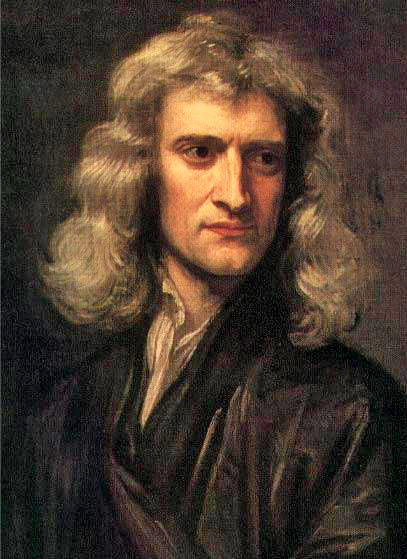
\includegraphics[scale=.25]{newton_portrait.jpg}

%\end{multicols}

}

% Section I:
\section{\sectiontitleI}

\frame{
\frametitle{\sectiontitleI}

The modeling process begins with a {\PR description} of the system and the modeling {\PN assumptions} that will be used. Typically a diagram of the system is included. \vspcc

%In rigid body motion, one {\B free body diagram} (FBD) per body is required for derivation of the {\G  equations of motion} of the system. 
% 
%However, the vector analysis of the forces involved is {\it not required} as it is in Newton's method. \vspcc


\underline{Question:} Why is the vector analysis not required for this method? 

%All forces that do {\OR work} on the sytem and all {\BR stored} energies storages m
	
}


% Section II:
\section{\sectiontitleII}

\frame{
\frametitle{\sectiontitleII}

After the model has been established, all kinetic energies associated with motion and all stored potential energies must be identified.  \vspc
\renewcommand{\arraystretch}{1.2}
\begin{tabular}{lll}
Kinetic Energy & &\\
&& \\
Potential Energy &&\\
&& \\
&&
\end{tabular}

\vspace{3mm}
A {\hspcu} \hspcu reference is required to properly define the potential energy function, $V(x)$.  


}



% Section III:
\section{\sectiontitleIII}

\frame{
\frametitle{\sectiontitleIII}

The conservation of energy can be used for deriving the dynamics (EOMs) for many systems. In some situations this is simpler that using Newton's method, however both methods will produce equivalent equations of motion. \vspc

\begin{framed}
\vspace{20mm}
%\renewcommand{\arraystretch}{1.2}
%\begin{tabular}{llc}
%%We know &\scalebox{1.0}{$ \Delta KE +\Delta PE = 0 $}& {\B(1)} \\
%%implies & \scalebox{1.0}{$ KE + PE = Constant $} & {\B(2)}\\
%%as well as & \scalebox{1}{$\frac{d}{dt}\left( KE + PE \right) = \frac{d}{dt}\left(Constant\right) = 0$} & {\B(3)}\\
%\end{tabular}
\end{framed}

We will use equation {\B(3)} to derive the equations of motion.

}


% Section IV:
\section{\sectiontitleIV}

\frame{
\frametitle{\sectiontitleIV}

You may recognize this problem from dynamics or physics class.\vspc However, today we will use the {\PR Conservation of Energy} to derive the equations of motion which contain the dynamic relationships between the system variables as functions of time.  \vspc

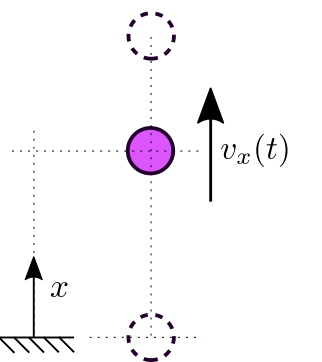
\includegraphics[scale=.3]{conservation_energy_fig2.png} 

\vspace{10mm}
{\tiny Images: T.Hill}
}

\frame{
\frametitle{\sectiontitleIV}

This a simple problem, but it shows the method clearly. To ensure correctness, validate the result with {\B Newton's Approach} \vspcc

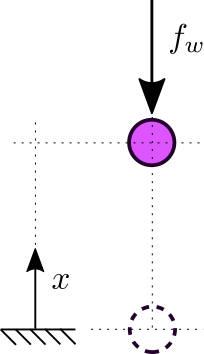
\includegraphics[scale=.3]{conservation_energy_fig3.png} 

\vspace{10mm}
{\tiny Images: T.Hill}
}
	
\end{document}





